\chapter{A Breakdown of all Completed Testing}

\section{Round 1 Testing: Initial Classifications}
\subsection*{Testing Considerations}

I began testing the tool with three main questions. I wanted to know how the accuracy of classification is affected by:

\begin{Spacing}{1.2}
\begin{itemize}
  \item The spatial distribution of pixels chosen to create the reference curves.
  \item The temporal distribution of pixels chosen to create the reference curves.
  \item The VI used for the classification.
\end{itemize}
\end{Spacing}

To test these factors, I chose six small sample areas dispersed across Kansas, each 100 MODIS pixels square, or about 2.3 KM$^2$ (Fig. \ref{fig:studysites}). Using the USDA CDL as reference, I identified areas containing a mix of corn, wheat, soy, sorghum, and winter wheat pixels. I did my best to distribute the small areas across the state to capture a wide variety of growing conditions. This task was surprisingly difficult, given the large extent of the state and the concomitant variation in growing conditions. The crops favored tended to change from one area to another; for example, few sites in western Kansas had little more than corn and wheat.

Within each sample site, I found four to eight MODIS pixels of each of the previously listed crop types. I took care to choose only pixels in the center of fields, under the assumption such pixels would be more representative of the crop’s true temporal signature. On each chosen pixel, I digitized a vector point feature, keeping points for each crop and study area in separate shapefiles  (Fig. \ref{fig:refpoints}). I used these shapefiles as inputs to the RSG, and created two sets of reference temporal signatures for each study area: one set from the NDVI MODIS data, and another from the EVI data. I also found the mean of the signatures identified for each crop in easy study area, which gave me mean NDVI and EVI reference temporal signatures averaged across all six study sites.

I classified both NDVI and EVI data for each of the sample areas using its own reference signatures, the reference signatures derived from each of the other sample areas, and the mean signatures from all of the sample areas. This allowed me to test how the spatial distribution of pixels used to construct reference signatures affects the accuracy of classification, and which of these two VIs performs better. My initial hypothesis was that averaging signatures across multiple sites would decrease the “truthfulness” of the reference signatures because of geographical discrepancies in season start date, maximum VI intensity, and/or season length. If reference signatures are usable between study areas, but averaging multiple sites together does in fact negatively affect the derived reference curves, I expected to see rather consistent classification accuracies independent of the reference signature set used, but that the mean reference signatures produced a lower classification accuracy than those derived from single sample sites. However, if reference signatures are not useable between study areas, I expected low accuracies when the reference signatures from different study areas are used for classification, while the mean reference signatures should perform somewhere between those of the study area in question and those of the other study areas. If spatial distribution has no effect, my expectations was that the classification accuracies would be relatively consistent no matter which reference signature set is used.

I knew these tests would not directly answer my question about temporal variation in the construction of reference temporal signatures. To get an accurate answer, I knew I would need to repeat the above testing, replacing location with time as the key variable. However, given my hypothesis about the effects of spatial variation, I wanted to find out my results before devising this test. If I found the spatial distribution of pixels negatively affected the classification accuracies, then I could reasonably conclude adding a temporal component would have a similar outcome, as temporal variance would also introduce discrepancies in season start date, maximum VI intensity, and/or season length. In such a case, additional testing of this parameter would not be necessary to proceed.

\begin{figure}
  \centering
  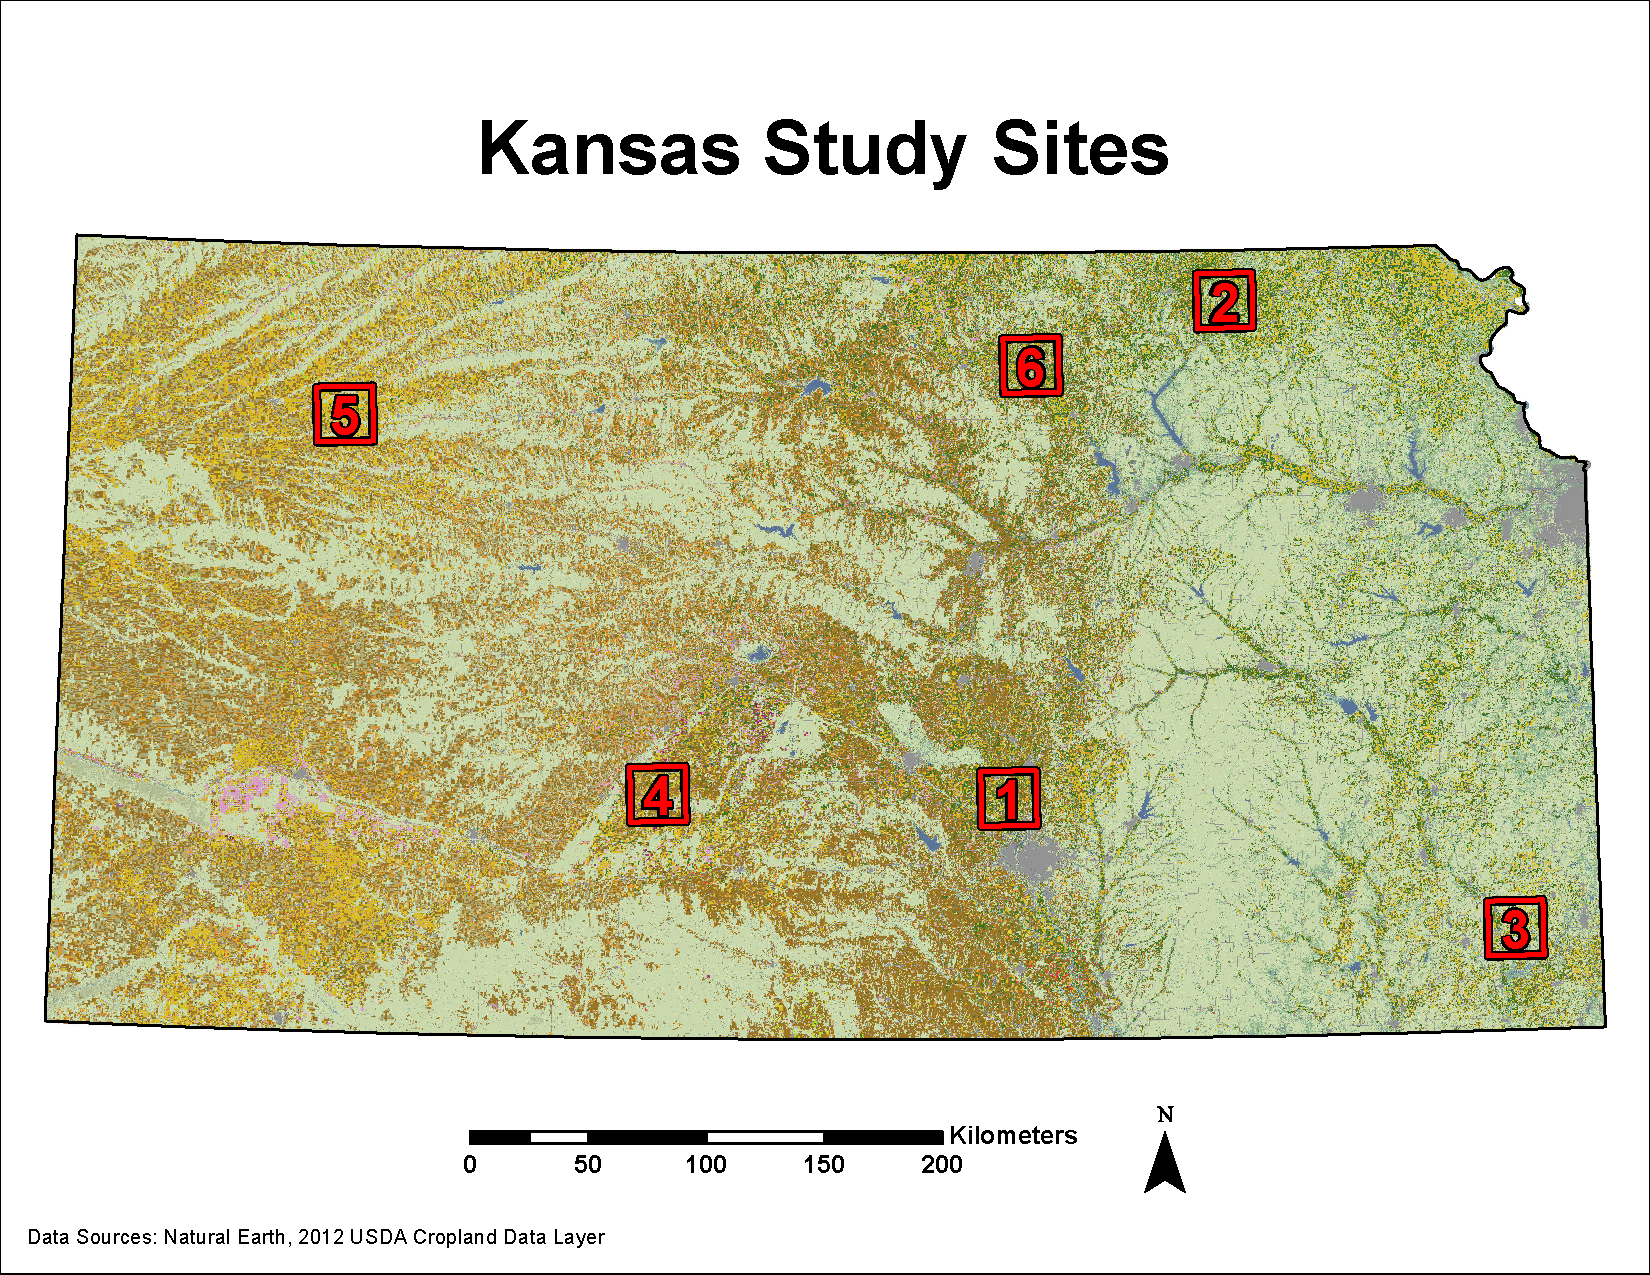
\includegraphics[width=.9\textwidth]{Graphics/Testing/STUDYSITES.pdf}
  \caption{The six study sites in Kansas.}
  \label{fig:studysites}
\end{figure}

\begin{figure}
  \centering
  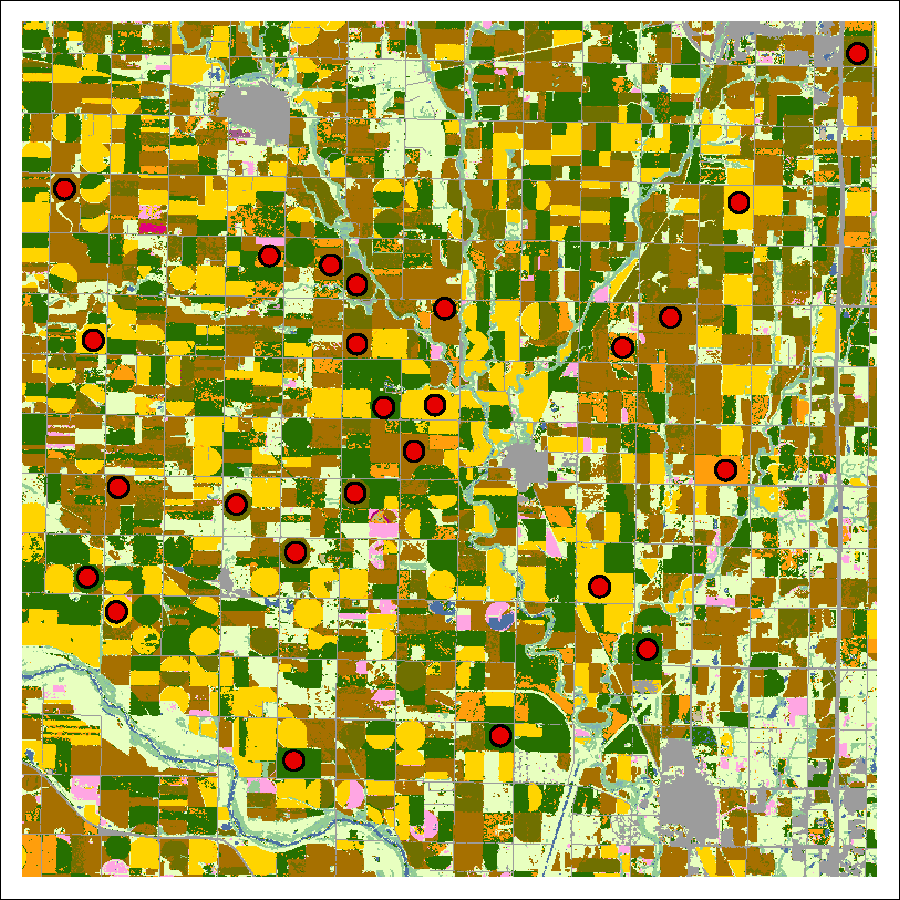
\includegraphics[width=.7\textwidth]{Graphics/Testing/clip1_30mCDL_smpl_old.pdf}
  \caption{Points dropped on pixels to use for reference signatures in study site 1.}
  \label{fig:refpoints}
\end{figure}

\subsection*{Round 1 Results and Discussion}

Some clear patterns pop out when reviewing Table \ref{table:round1results}. First, a quick scan of all the values shows that none of the classifications had a very high degree of accuracy, though study site 3 stands out with much higher accuracies than the rest. A more detailed examination of of study site 3’s results shows that the increased accuracy is due to the fact that relatively few of the pixels in the sample site are crop pixels, and a high accuracy can be achieved by not classifying the majority of the pixels, such that they are considered “other.” A breakdown of highest accuracy sample site 3 classification, that using sample site 3’s reference signatures and NDVI data, is shown in Table \ref{table:round1ss3acc}. One can see the relative abundance of “other” pixels that skews the accuracy upward compared to the other sample sites.

\begin{Spacing}{1.0}
\begin{table}
  \centering
  \caption{Overall Percent Accuracy for Each Round 1 Classification, by Sample Site (SS).\newline~Green cells indicate highest accuracy for each sample site.}
  \label{table:round1results}
  \begin{tabu}{ZZZZZZZZ}
    \toprule
    \multicolumn{8}{c}{\textbf{EVI}} \\
    \midrule
    & \multicolumn{7}{c}{Reference Signatures Source} \\
    & SS 1 & SS 2 & SS 3 & SS 4 & SS 5 & SS 6 & Mean \\
    \midrule
    SS 1 & \cellcolor{LimeGreen}55.61 & & 45.34 & 54.36 & 43.83 & 49.06 & 49.63\\
    \rowcolor{light-gray}SS 2 & 53.11 & \cellcolor{LimeGreen}64.93 & 50.00 & 47.86 & 40.79 & 42.60 & 53.69 \\
    SS 3 & 73.87 & 69.40 & \cellcolor{LimeGreen}75.23 & 73.53 & 70.57 & 71.86 & 73.71 \\
    \rowcolor{light-gray}SS 4 & 50.42 & 45.54 & 49.26 & \cellcolor{LimeGreen}53.46 & 45.30 & 49.66 & 52.54 \\
    SS 5 & 42.05 & 45.62 & \cellcolor{LimeGreen}56.00 & 54.68 & 55.06 & 49.02 & 40.29 \\
    \rowcolor{light-gray}SS 6 & 47.78 & 48.66 & 38.43 & 47.53 & 41.60 & \cellcolor{LimeGreen}49.55 & 48.44 \\
    \bottomrule
    & & & & & & & \\
    & & & & & & & \\
    \toprule
    \multicolumn{8}{c}{\textbf{NDVI}} \\
    \midrule
    & \multicolumn{7}{c}{Reference Signatures Source} \\
    & SS 1 & SS 2 & SS 3 & SS 4 & SS 5 & SS 6 & Mean \\
    \midrule
    SS 1 & \cellcolor{LimeGreen}61.08 & 48.29 & 47.91 & 60.72 & 44.85 & 51.81 & 52.75 \\
    \rowcolor{light-gray}SS 2 & 56.08 & \cellcolor{LimeGreen}67.39 & 42.66 & 52.59 & 50.62 & 48.95 & 61.21 \\
    SS 3 & 74.88 & 71.75 & \cellcolor{LimeGreen}78.69 & 77.16 & 70.62 & 71.75 & 73.70 \\
    \rowcolor{light-gray}SS 4 & 56.30 & 42.25 & 46.89 & \cellcolor{LimeGreen}59.21 & 44.72 & 54.26 & 52.48 \\
    SS 5 & 53.57 & 48.51 & 45.93 & 62.18 & \cellcolor{LimeGreen}62.83 & 60.21 & 53.07 \\
    \rowcolor{light-gray}SS 6 & & 51.90 & 38.28 & 49.82 & 47.15 & \cellcolor{LimeGreen}55.71 & 54.36 \\
    \bottomrule
  \end{tabu}
\end{table}
\end{Spacing}

[INCLUDE THE TOP ACCURACIES OF EACH OF THE OTHER SAMPLE SITES IN TABLES]

\begin{Spacing}{1.0}
\begin{table}
  \centering
  \caption{Sample site 3 NDVI top accuracy}
  \label{table:round1ss3acc}
  \begin{tabu}{rrrrrrl}
    \toprule
     & Corn & Soy & Wheat & Other & Total & User Accuracy \\
    \midrule
    Corn & 861 & 133 & 0 & 334 & 1328 & 65\% \\
    Soy & 28 & 558 & 13 & 198 & 797 & 70\% \\
    Wheat & 2 & 4 & 23 & 37 & 66 & 35\% \\
    Other & 884 & 424 & 74 & 6427 & 7809 & 82\% \\
    Total & 1775 & 1119 & 110 & 6996 & &  \\
    Producer Accuracy & 49\% & 50\% & 21\% & 92\% &  &  \\
     &  &  &  & \multicolumn{3}{r}{Overall Accuracy: 79\%} \\
     &  &  &  & \multicolumn{3}{r}{Kappa: 0.49} \\   
    \bottomrule
  \end{tabu}
\end{table}
\end{Spacing}

Another pattern that stands out is that using NDVI resulted in a higher top accuracy for every sample site. The numbers are fairly close between the two, so I am hesitant to conclude that optimizations would fail to make EVI-based classifications as or more accurate than NDVI-based classifications. Nonetheless, based on these results, I have determined to continue testing with NDVI only, as it seems to perform better.

Perhaps most striking pattern in Table \ref{table:round1results} is that, aside from sample site 5 in the EVI-based classifications, the highest accuracies occurred when the reference signatures generated from a particular study site were used to classify that same study site. This is not wholly unexpected—even if temporal signatures are largely location-independent, there is likely to be some location-specific phenomena influencing the shape of the signature curves. In some cases, it appears that some of the classifications using other reference signatures were of similar accuracy, as occurs with sample site 1 when it is classified using sample site 4’s signatures (61.1 percent versus 60.7 percent). However, in other cases, the accuracy is marked lower, exemplified by sample site 1 when it is classified using signatures from sample sites 2, 3, 5, and 6 (all are around ten percent lower in accuracy).

The accuracies of the mean reference signature classifications are generally low. They are never the worst, which may suggest that it is better to average a greater number of pixels together if the representative-ness of the chosen pixels cannot be established. However, this conclusion would support a more selective and refined approach to creating reference signatures: don’t try to average out bad pixels, eliminate them in the first place.

Looking back on the scenarios I outlined in my testing considerations above, I actually found none of them completely captured the behavior shown in the results. I did not see relatively consistent classification accuracies independent of the set of reference signatures used, but I also found that the reference signatures from some sample sites did well at classifying others. The mean signatures were also somewhat in the middle, generally not doing terribly well, but sometimes coming close. The best interpretation I could make of the results is that, under the right circumstances, reference signatures can be used to classify other areas. However, the cases where the reference signatures are not portable, in addition to the low overall accuracy levels, were concerning. I began to consider that I might not be able to answer the initial testing questions; instead, I realized I needed to take a step back and better explore what factors effect the classification process.

\section{Round 2 Testing: Eliminating Mixels}
\subsection*{Pre-testing Investigation}

I began my Round 2 testing by diving back into my Round 1 results. I wasn’t sure exactly what I needed to test, but I knew my previous results held more clues. For the sake of simplifying my investigation, I decided to focus solely on sample site 1 for the remainder of my testing. If I could boost the accuracy of its classification, I would identify some of the factors influential in the classification process. I chose sample site 1 over the others as it has the best variety of crops in which I am interested, and also includes some large non-crop areas of different land cover types. This mix seemed to offer the best testing environment of my six sites.

I first studied the classification results for sample site 1 from Round 1 produced with its own reference signatures (Fig. \ref{fig:ss1r1class}). I noticed that the major patterns generally matched the CDL fairly well. If the classification \textit{looks} correct, however, where were the errors? Obviously there should be many incorrect pixels, as this classification only had an accuracy of about 61 percent. Yet they weren’t obvious at first glance.

\begin{figure}
  \centering
  \begin{subfigure}[b]{.45\textwidth}
    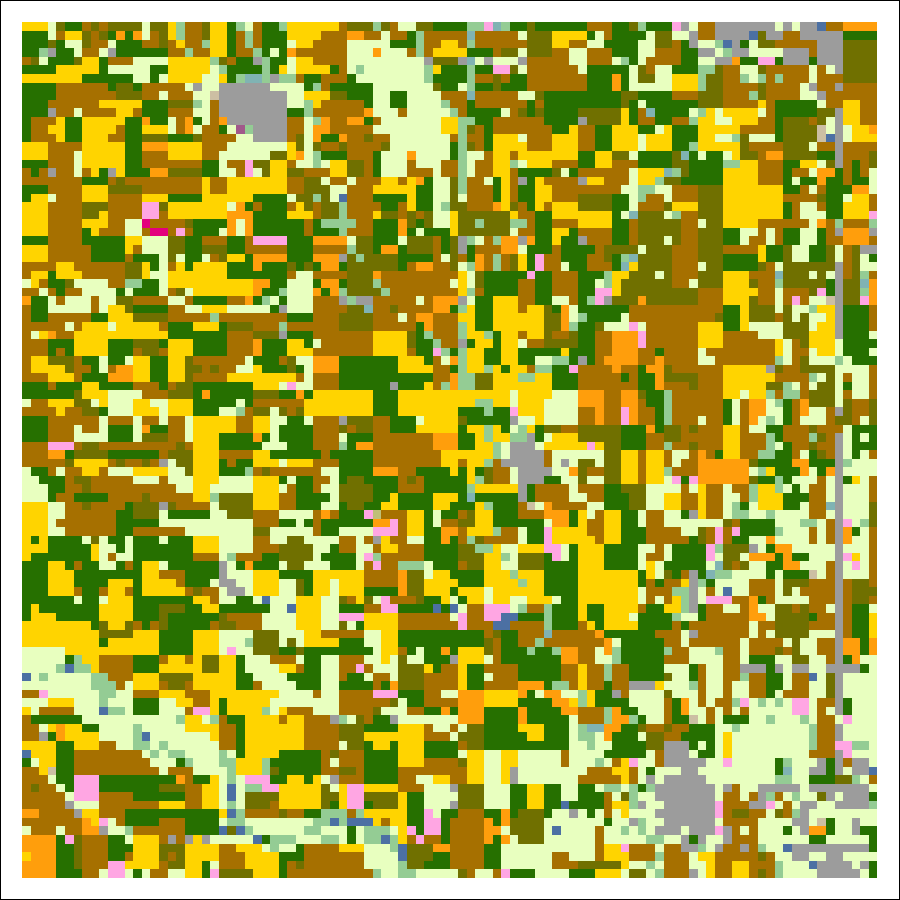
\includegraphics[width=\textwidth]{Graphics/Testing/clip1_MODIS_CDL.pdf}
    \caption{The 2012 CDL.}
    \label{subfig:ss1r1CDL}
  \end{subfigure}
  \quad
  \begin{subfigure}[b]{.45\textwidth}
    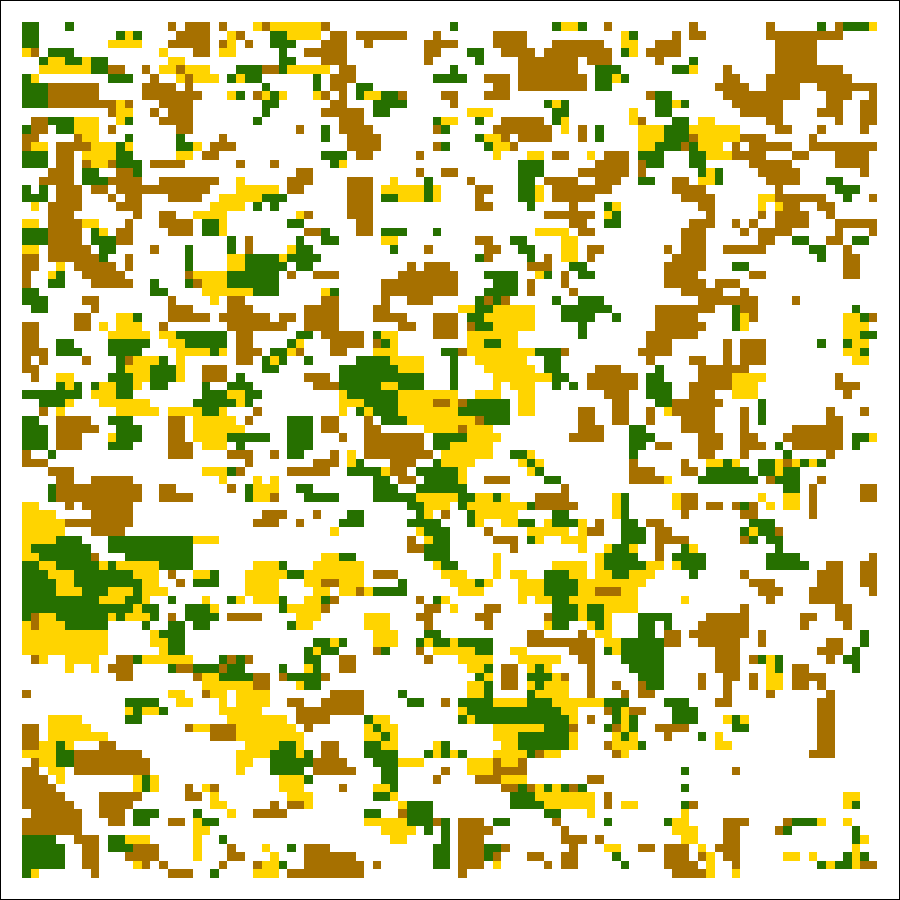
\includegraphics[width=\textwidth]{Graphics/Testing/clip1_MODIS_round1.pdf}
    \caption{Round 1 classification using SS 1 signatures.}
    \label{subfig:ss1r1class}
  \end{subfigure}
  \\
  \vspace{.25in}
  \begin{subfigure}[b]{.45\textwidth}
    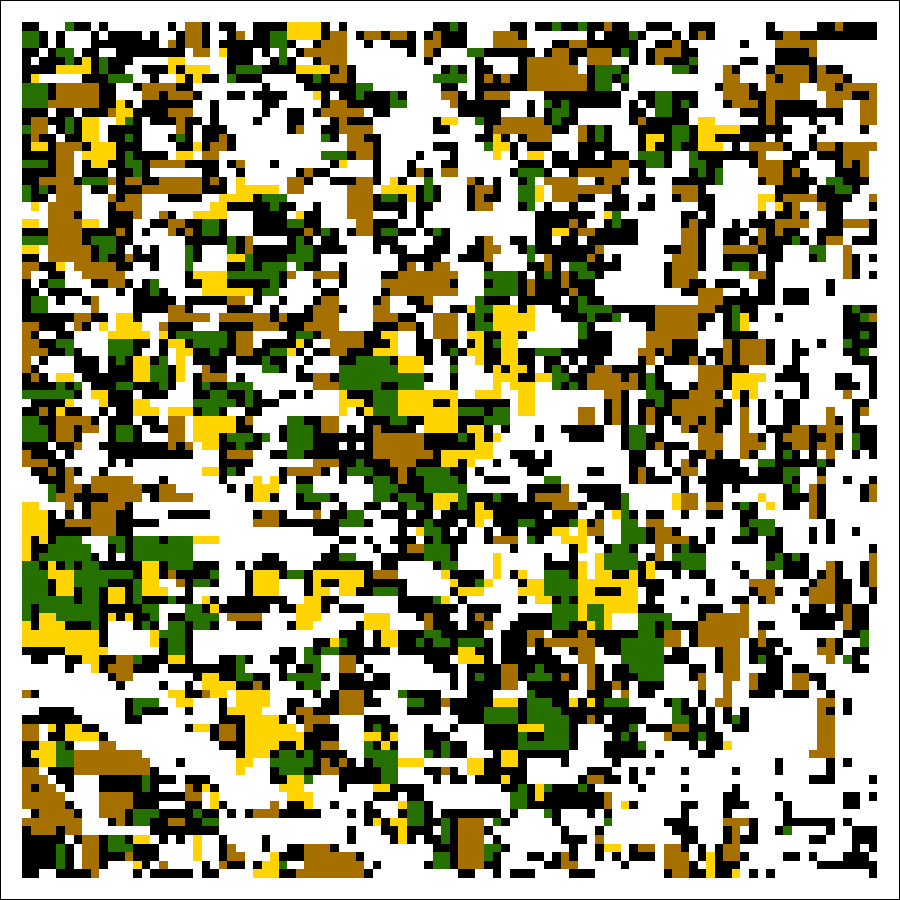
\includegraphics[width=\textwidth]{Graphics/Testing/clip1_MODIS_round1_correct.pdf}
    \caption{Correctly classified pixels. Incorrect pixels in black.}
    \label{subfig:ss1r1correct}
  \end{subfigure}
  \quad
  \begin{subfigure}[b]{.45\textwidth}
    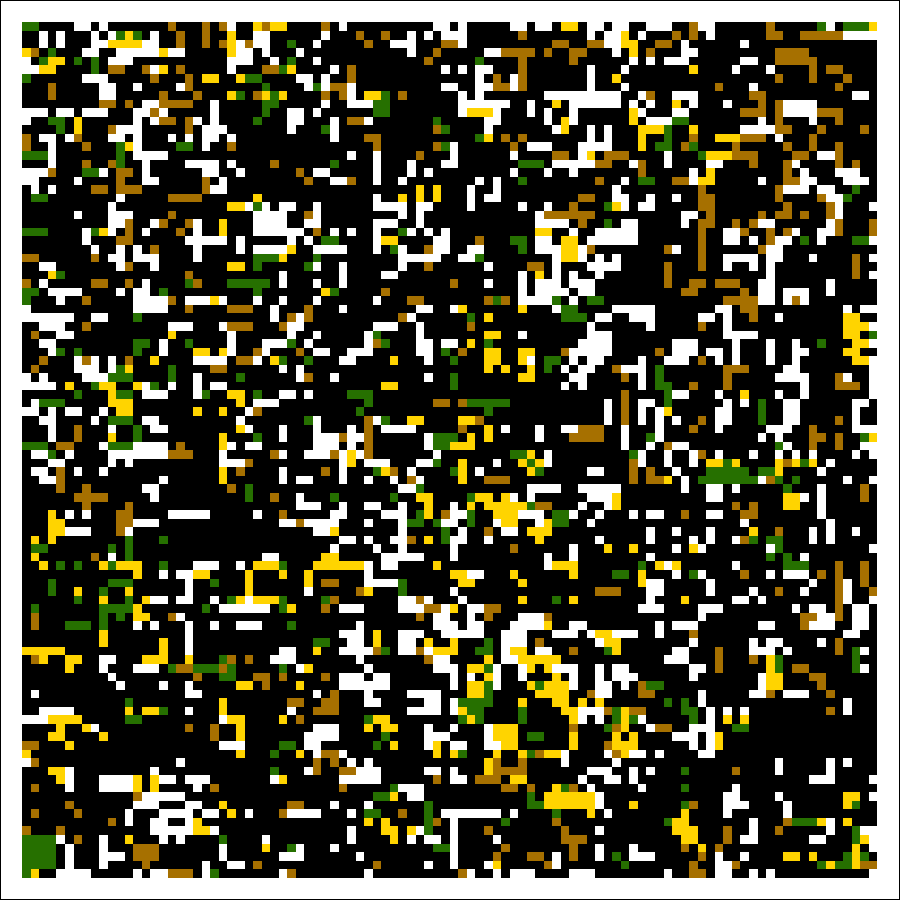
\includegraphics[width=\textwidth]{Graphics/Testing/clip1_MODIS_round1_incorrect.pdf}
    \caption{Incorrectly classified pixels. Correct pixels in black.}
    \label{subfig:ss1r1incorrect}
  \end{subfigure}
  \caption{Sample Site 1, Round 1 classification.}
  \label{fig:ss1r1class}
\end{figure}

To find these incorrect pixels, I created two images: an image with the incorrect pixels masked in black, and an image with the correct pixels masked in black (Figs. \ref{subfig:ss1r1correct} and \ref{subfig:ss1r1incorrect}). In the former, I noticed that many of the incorrect pixels seemed to fall on the edges of fields. In the latter, I noticed some class confusion, a finding reinforced by the confusion matrix for this classification (Table \ref{table:ss1r1acc}).

The class confusion seemed to be a problem, but how to begin to remedy it was not immediately obvious to me. That so many border pixels were incorrectly classified, conversely, suggested to me that this classification method struggles when pixels have more than one land cover. Such pixels are often termed mixels.

The problem with mixels is that each land cover in a mixel has a different temporal signature. The different signatures are aggregated at the pixel level and become mixed, creating a new signature representing that specific mixture of individual signatures. This problem is not unique to my temporal data; all raster land cover data has mixels. Users of spectral data even have spectral unmixing tools to extract subpixel spectral information [CITATION].

In my case, the large size of the MODIS pixels increases their possible effect on classification accuracy. Many different land covers can be included within a 232-meter square. The large pixel size also means that a much greater percentage of the study area is composed of mixels than if a smaller pixel were used.

For these reasons, I hypothesized the low classification accuracy was becasue mixels could not be processed accurately by the fit algorithm due to the contaminated signal in a mixel curve. In other words, if two crops are mixed within a pixel, the curve of that pixel’s values from the time series image will be a blend of both crops’ phonological curves, and neither will have a good fit. Additionally, the crop which may occupy the majority of the area of the pixel may not be the largest contributor a pixel’s values; for instance, due to its high maximum VI values, a crop like soy may drive a pixel’s values up at the time of the year it is mature, even if it is in the minority of the pixel. This would further reduce the accuracy when compared to the CDL resampled by majority. Consequently, I determined I needed to find a way to removed mixels from the classification.

\subsection*{The Testing Process}

The first step in removing the mixels was to extract the MODIS raster grid from the sample site 1 TSI as vector polygons. The CDL raster is of sufficient spatial resolution (30-meter) to allow identification of fields; I converted the CDL to vector, and all continuous pixels of the same land cover value were merged into single vector features. Next, I intersected these CDL features with the pixel polygon features of the MODIS grid. From the resulting vector features I was able to select only those with an area close to that of a full MODIS pixel. Specifically, I decided to select all features greater than or equal to 53,000 m$^2$ in area (a full MODIS pixel being 53,824 m$^2$). I also manually added two [CHECK THIS] sorghum pixel features that were not selected via this process because of the low number of sorghum pixels retained. The result, shown in Fig. \ref{fig:ss1purepx}, was [INSERT NUMBER OF FEATURES HERE] features selected. These features can be thought to represent MODIS pixels which have “pure” signatures: each pixel has only one land cover contributing to its temporal signature, so each should be representative of its class.

\begin{figure}
  \centering
  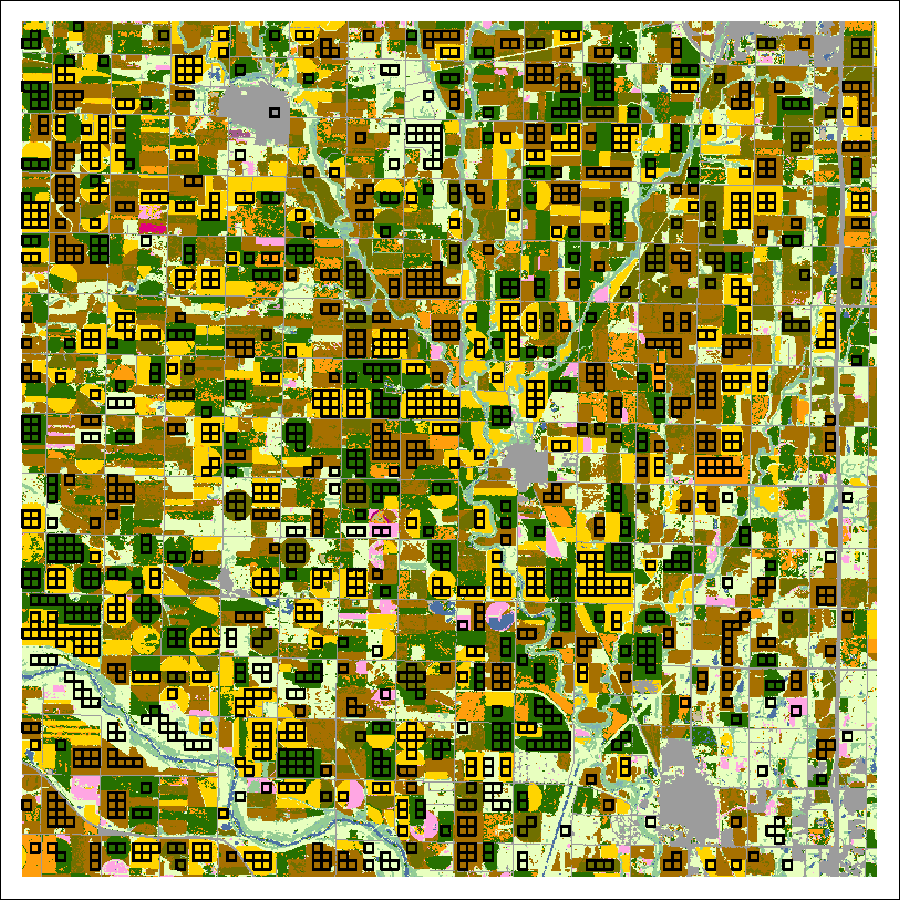
\includegraphics[width=.7\textwidth]{Graphics/Testing/clip1_30mCDL_pure_pixels.pdf}
  \caption{The pure pixels in Study Site 1.}
  \label{fig:ss1purepx}
\end{figure}

To allow me to classify only these pure pixels, I found the centroid of each of the selected pixel polygon features. The subset option of the Find Fit Tool allowed me to specify a shapefile of point features, which were converted to a list of pixel coordinates from the TSI; the tool then found the fit of the pixels in this list only. All the other pixels were assigned the  no data value. All other classification steps were the same as in Round 1, except the no data values in the fit rasters were ignored by the Classify tool when considering accuracy.